\documentclass[11pt]{article}
\usepackage{amsmath, amssymb}
\usepackage{graphicx}
\usepackage{float}
\usepackage{hyperref}
\usepackage{cite}
\usepackage[margin=1in]{geometry}


\title{A Simple MNIST Digit Classifier Neural Network Made from scratch in Python}
\author{Thiruwaran Kalvin (T-Kalv) \\
Undergraduate Computer Science Student}
\date{\today}

\begin{document}

\maketitle

\section{Abstract}
This research paper presents an implementation of a basic feed-forward neural network for classifying/recognising handwritten digits from the MNIST dataset, built from scratch in Python using only core libraries such as NumPy, Matplotlib, Pandas, and tqdm. This feed-forward neural network model, also known as a multilayer perceptron (MLP), achieves a classification probability accuracy of appoximately 88\% for both the training and testing datasets. This demonstrates the viability of simple neural networks that recognise handwritten numerical digits without the need for external heavy libraries such as PyTorch or TensorFlow, instead utilising only core Python libraries and Juypter Notebook.

\section{Introduction}
Numerical Digit Classification is a specific field of Image Processing that focuses here on this paper, classifying and recognising handwritten low-level black and white numerical digit images using the MNIST Dataset[1]. This particular task of recognising handwritten digits is vital in the real-world as previously Bank Tellers played a crucial role in processing Cheques by manually verifying (looking) at the authenticity of the Cheques and verifying the Currency amount on the Cheques. This method was time-consuming and in-efficient due to manual Human validation as well as being prone to Human errors. As the level of technology/computation advanced, the need to accurately read hand-written numerical digits especially in sectors such as the Banking industry became more crucial to reduce the likelyhood of errors and reduce processing time. This results in Financial institutions diversting resources more effectivly to other services. Through the advancements in Artificial Intelligence and Machine learning, we can develop systems that can accuracy recognise hand-written digits much more efficient and effectively using hand-written datasets such as MNIST.

\vspace{1em}
%https://en.wikipedia.org/wiki/MNIST_database#cite_note-yadav2019-23
MNSIT (Modified Natual Institute of Standard and Technology) database is dataset that consits of handwritten numerical digits that is commonly used for image processing training and contains 60,000 training images used to train the Machine Learning Neural Network model and 10,000 testing images to validate the accuracy of the model. In this paper, we use this famous MNIST dataset which is the standard benchbark for Image Classification algorithms. As the MNIST database was constructed before the turn of the 21st Century, there have many implementations/existing solutions using the MNIST Dataset to classify and recognise hand-written numerical digits such as using tradition methods (including but not limited to KNN (K-Nearest Neighbours), SVM (Support Vector Machines)) and even Deep-Learning methods (including but not limited to CNN (Convultional Neural Network), RNN (Recurrent Neural Network)). Arguably, one of the most famous implementations it the LeNet-5 architecture [3] which uses CNN consiting of 2 convolutions, 2 subsamplings and 3 fully connected layers with around 60000 trainable paramaters.

\vspace{1em}
This paper proposes a light-weight simple MNIST Digit Classifier Neural Network [4] consiting of 2 layers with 784 neurons, built without the use of external heavy deep-learning libraries  (only using libraries such as NumPy, Matplotlib) with a particular emphasis on understanding and manually implementing algorithms and functions. This work presents such algorithms and functions such as Forward Propagation, Backpropagation, ReLu (Rectified Linear unit) activation function, Softmax activation function\dots. This results in a reproducible implementation of simple MNSIT Digit Classifier Neural Network, with clear, hand-on demonstration of 'behind-the-scenes' of the network as well as the training procedure and performance benefits/outcomes.

\vspace{1em}
This paper is organised as follows: Section 3 discusses related work, followed by Section 4 which outlines the Methodology and architecture, Section 5 presents Experimental Evaluation and finally Section 6 concludes with findings and future work.


\section{Related Work}
% TODO: Discuss related papers and prior work.
Before working on this 'Simple MNIST Digit Classifier Neural Network', previously a 'Simple Neural Network' was developed from scratch in Python for XOR [4]. This previous project implemented key concepts such as Forward Propagation, Backpropagation, Mean-Squared Error Loss and the Sigmoid Activation function using only core libraries such as NumPy and Matplotlib. The sucess of XOR having a probability of appoximately 95\% helped to inspire the next challenge of handling a more real-world dataset MNIST, implementing these key concepts on this 'Simple MNSIT Digit Classifier Neural Network'.

\vspace{1em}
%https://axon.cs.byu.edu/~martinez/classes/678/Papers/Convolution_nets.pdf
Previous research into using the MNIST dataset for classifying and recognising handwritten digits has produced a wide-range of models with a variety of complexity and performance benefits to the traditional manual, human-validation of handwritten digits. LeNet-5 [3], introduced in 1998 having achived appoximately a 1\%[5] test error probability which resulted in appoximatly 99\% probability accuracy with the MNSIT dataset, implemented using CNN (Convultional Neural Networks). While LeNET-5[5], achived a respectable, high probability accuracy using CNN, Max Pooling with 2 convultions, 2 subsampling, 3 fully connected layers and around 60000 trainable paramaters, this paper investigates the performance of a simple multilayer perceptron (MLP) using a feed-forward neutal network trained from scratch without the need of heavy, high-level frameworks. However, more modern implementations do use these heavy, high-level frameworks such as PyTorch [6], Keras [7], TensorFlow [8] utilising the performance benefits of GPUs (Graphics Processing Unit), NPU (Neural Processing Unit), TPUs (Tensor Processing Units) which help to optimise the speed of learning/training as well with the use of advanced optimisers (including but not limited to Adam). Here due to the added cost of utilising such performance enhancers, the system here presented in this paper will instead utilise modern CPUs for computation and training.

\section{Methodology}
\subsection{Dataset}
\begin{figure}[H]
  \centering
  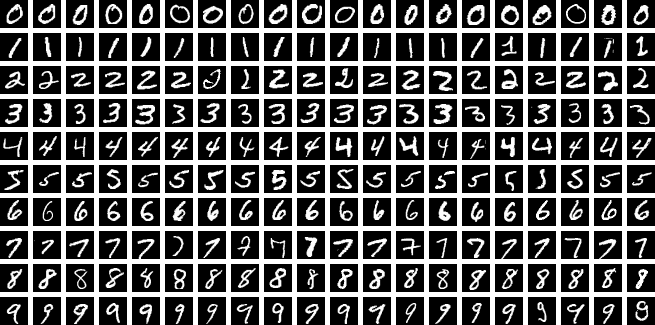
\includegraphics[width=0.6\textwidth]{MNIST_dataset_example.png}
  \caption{Sample handwritten digits from the MNIST dataset. Image by Suvanjanprasai, CC BY-SA 4.0.}
  \label{fig:mnist}
\end{figure}

%kaggle mnist dataset
%image of mnist numbers - By Suvanjanprasai - Own work, CC BY-SA 4.0, https://commons.wikimedia.org/w/index.php?curid=156115980
The MNIST dataset [9] contains gray-scale, black and white images of hand-drawn numerical digits from zero to nine (0, 1, 2, 3, 4, 5, 6, 7, 8, 9). Each image is 28 pixels in height by 28 pixels in width) contains a total of 784 pixels, where each pixel value is an integer from 0 to 255 resulting in black to white. The dataset consits of 60000 training images for training the model and 10000 testing images for testing the trained model. The training dataset in this paper has 785 columns which are the 'label'. This is the corresponding '0 to 9' digit that was handwritten and the remaining columns are the '0 to 255' pixel values associated with the black and white image. The testing dataset is the same as the training dataset execept without containing the labels to validate the accuracy of the model.


\subsection{Network Architecture}
\begin{figure}[H]
  \centering
  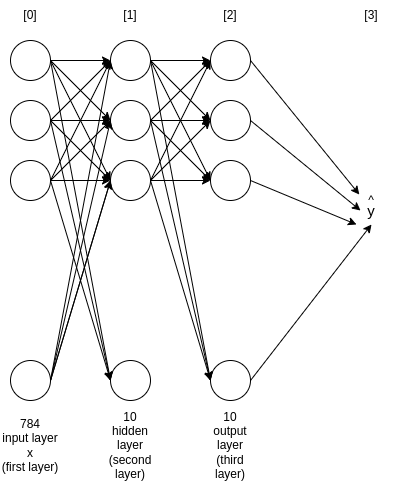
\includegraphics[width=0.6\textwidth]{Neural Network.drawio.png}
  \caption{Simplified Neural Network Architecture used in this Project}
  \label{fig:mnist}
\end{figure}

The Neural Network [Figure 2] is a fully-connected, feed-forward neural network that consits of an input layer, hidden layer and output layer. The input layer (first layer x) consits of 784 neurons which correspons to the 784 pixels in the 28x28 flattened image for each of the images in the MNSIT dataset. The hidden layer (second layer) consits of 10 neurons where the corresponding weights and biases connecting to this layer and initialised with random values between -0.5 to 0.5. In addition, the activiation function used in the hidden layer is the ReLu (Rectified Linear unit) activation function. The output layer (third layer) consits of 10 neurons which is the precition of what numerical digit the input image represents from 0 to 9 resulting in 10 possible numerical digit classes.

\vspace{1em}
The parameters of this Neural Network consits of a 'weight1' which has a shape of (10,784) connecting the input to the hidden layer, 'bias 1' which has a shape of (10,1) which are the biases for the hidden layer, 'weight 2' which has a shape (10,10) connecting the hidden layer to the output layer and 'bias2' which has a shape of (10,1) which are the biases of the output layer. This results in this simple MNIST Digit Classifier Neural Network having a total of 7960 trainable parameters with 7840 weights, 10 biases between the input layer and hidden layer, 100 weights, 10 biases between the hidden layer and putput layer.

\subsection{Forward Propagation}
% TODO: Explain forward pass.

\subsection{Backpropagation and Loss Function}
% TODO: Explain backward pass and loss.

\subsection{Training}
% TODO: Describe training loop and parameters.

\section{Experimental Evaluation}
\subsection{Accuracy Results}
% TODO: Report performance metrics.

\subsection{Observations}
% TODO: Discuss what you saw.

\subsection{Limitations and Anomalies}
% TODO: Mention issues or incorrect predictions.

\section{Conclusion and Future Work}
% TODO: Wrap up the paper and list ideas for improvement.

\appendix
\section*{Appendix}
% TODO: Add any code snippets or extra figures.

\begin{thebibliography}{9}
% TODO: Add citations here.
\end{thebibliography}

\end{document}
